\section{ATLAS Coordinate System} \label{sec:atlas:coordinates}

Choosing the nominal interaction point as the origin, ATLAS defines a right-handed
coordinate system where the positive $x$-axis points towards the center of the
LHC ring, the positive $y$-axis points upwards, and the positive $z$-axis is
defined by the counter-clockwise circulating beam direction as viewed from
above, as shown in \Cref{fig:atlas_geometry} \cite{PERF-2007-01}.  
 
\begin{figure}[!htbp]
  \begin{center}
    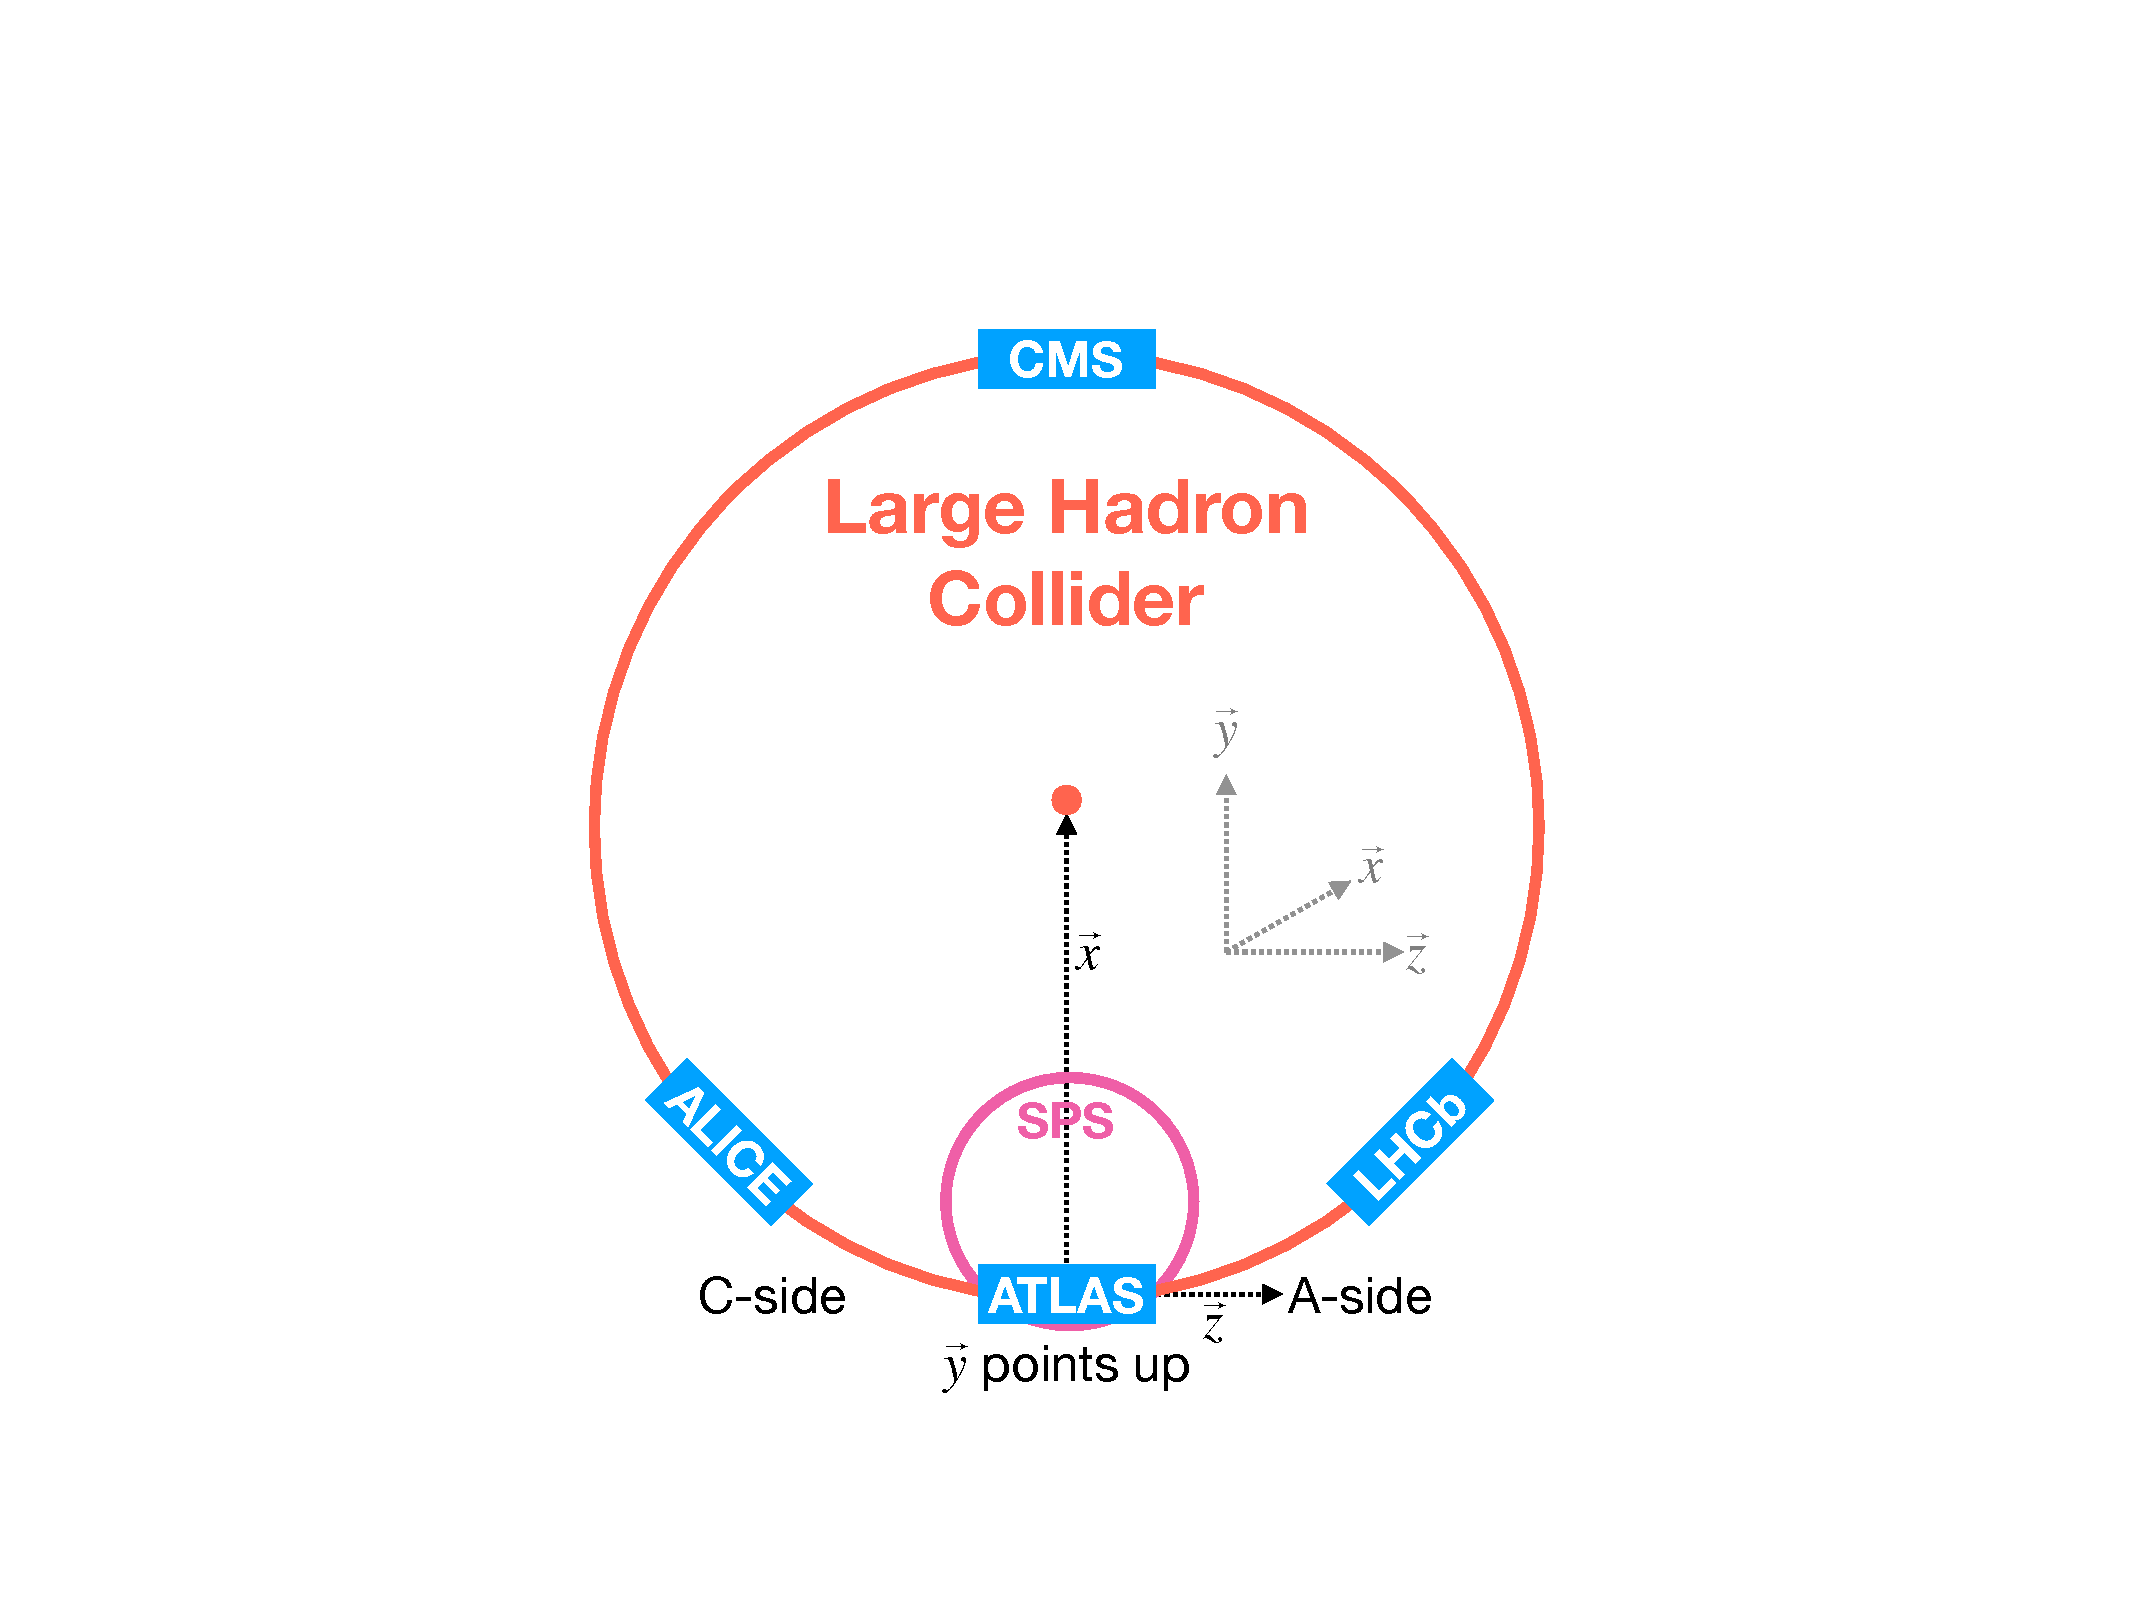
\includegraphics[width=0.7\linewidth]{figures/atlas/atlas_geometry}
    \caption{ The standard Cartesian coordinate system is shown with its origin at
the ATLAS interaction point, the positive $x$-axis towards the center of the
LHC, the positive $y$-axis pointing upwards, and the positive $z$-axis pointing
along the beamline \cite{Feickert:2690521}.}
    \label{fig:atlas_geometry}
  \end{center}
\end{figure}

Using these coordinates the physical momentum of the objects measured is
defined as $\vec{p} = (\pt,p_z)$ with \pt being the momentum of the object in
the transverse plane and $p_z$ the momentum along the beam axis. Considering
the cylindrical symmetry of ATLAS it is desirable to define the polar angle
$\theta$ from the beam axis with the $r$-$\phi$ plane being perpendicular to
that axis.  The radial distance is defined as $r = \sqrt{x^2+y^2}$ and the
azimuthal angle is defined with $\phi = 0$ corresponding to the $x$-axis.

The initial state of a collision is inevitably boosted in the $z$-axis, but
it is difficult to accurately measure this boost. Instead it is preferable to use
geometric quantities which are invariant under these boosts. In the high energy
regime, the pseudorapidity 

\begin{equation}
 \eta = -\ln \tan \left( \frac{\theta}{2} \right)
\end{equation}

is a good approximation of the rapidity ($y$) of a particle --- a measurement of
the velocity of a particle parallel to the beam axis ($z$-axis)

\begin{equation}
y = \frac{1}{2} \ln \left( \frac{E + p_{z}}{E - p_{z}} \right)
\end{equation}

where $E$ is the energy of the particle and $p_{z}$ is defined above.
Differences in rapidity ($\Delta y$) are Lorentz invariant under boosts along
the $z$-axis.  However, pseudorapidity is preferred as it is an entirely
geometric quantity independent of particle energy. \Cref{fig:pseudorapidity}
gives a sense of the distribution of $\eta$ in the $y$-$z$ plane. Since $\phi$
is defined in the $x$-$y$ plane, differences in the azimuthal angle
($\Delta\phi$) are also invariant under Lorentz boosts along the $z$-axis.
This allows for the definition of the functionally Lorentz invariant angular
separation

\begin{equation}
 \DeltaRdef \,
\end{equation}

between objects in the detector.

\begin{figure}[!htbp]
  \begin{center}
    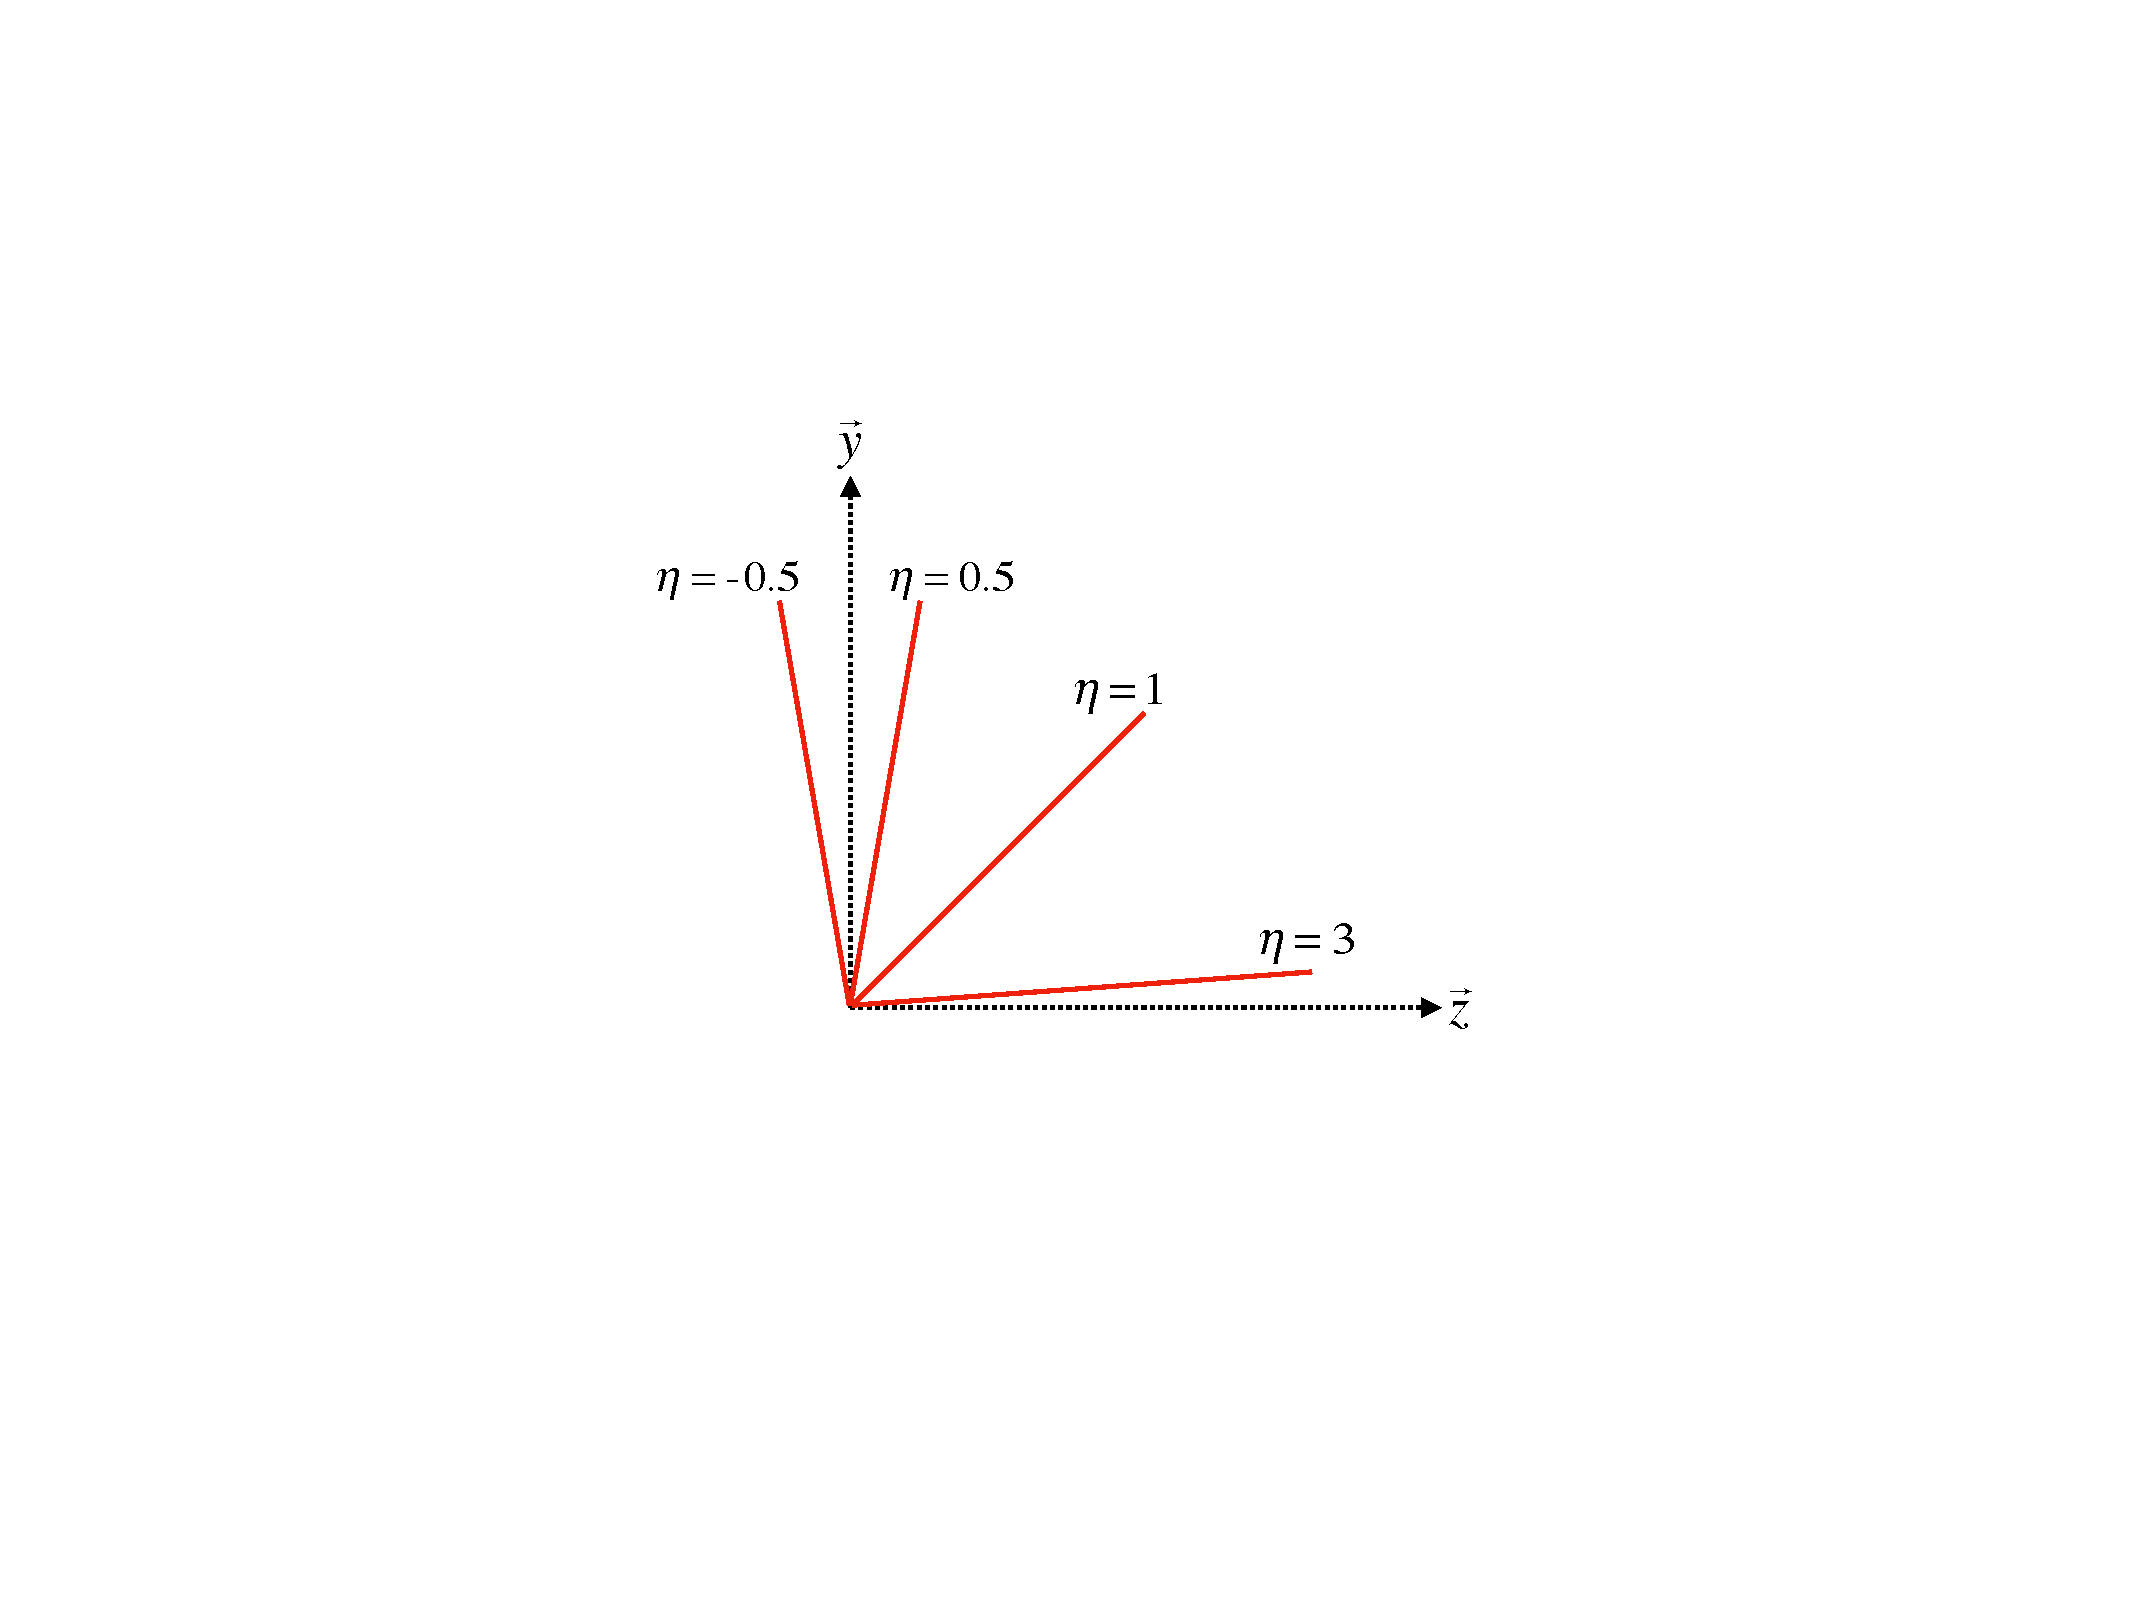
\includegraphics[width=0.5\linewidth]{figures/atlas/pseudorapidity}
    \caption{Modified from \cite{Stark:2317296} this cartoon represents a
selection of pseudorapidity $(\eta)$ values overlaid with some Cartesian
coordinates (dashed black lines).  The red lines are drawn for $\eta = \pm
0.5, \; 1.0 \text{ and } 3.0$.}
    \label{fig:pseudorapidity}
  \end{center}
\end{figure}

